\documentclass[11pt]{article}

\usepackage[a4paper,margin=25mm]{geometry}
\usepackage[T1]{fontenc}
\usepackage[utf8]{inputenc}
\usepackage{lmodern}
\usepackage{microtype}
\usepackage{amsmath,amssymb,bm}
\usepackage{booktabs,tabularx,array}
\usepackage{placeins}
\usepackage{siunitx}
\usepackage{graphicx}
\usepackage{xcolor}
\usepackage{tikz}
\usetikzlibrary{arrows.meta,positioning,fit,backgrounds,calc}
\usepackage[round,authoryear]{natbib}
\usepackage{xurl}
\usepackage[colorlinks=true,allcolors=blue!55!black,
  pdftitle={Dynamical Calibration of a Metallicity-Dependent Mass--Luminosity Relation from Gaia Wide Binaries}]{hyperref}
\usepackage[nameinlink,noabbrev]{cleveref}

\newcommand{\mh}{[\mathrm{M}/\mathrm{H}]}
\newcommand{\msun}{M_{\odot}}
\newcommand{\Normal}{\mathcal{N}}
\newcommand{\StudentT}{\mathcal{T}}
\newcommand{\indicator}{\mathbb{I}}
\newcommand{\softplus}{\operatorname{softplus}}
\newcommand{\sigmoid}{\operatorname{sigmoid}}
\newcommand{\dd}{\,\mathrm{d}}
\newcommand{\kmsau}{\mathrm{km}\,\mathrm{s}^{-1}\sqrt{\mathrm{AU}}}

\title{Dynamical Calibration of a Metallicity-Dependent Mass--Luminosity Relation\\
from Gaia Wide Binaries}
\author{}
\date{Frozen model configuration: 13 September 2026}

\begin{document}
\maketitle

\section{Scientific objective and modular architecture}
\label{sec:overview}

The aim is to infer the stellar mass $M$ as a function of Gaia absolute
$G$-band magnitude $x\equiv M_G$ and metallicity $Z\equiv\mh$, while retaining
the astrophysical mass scale supplied by the PARSEC stellar-evolution models
\citep{Bressan2012PARSEC}.  Wide binaries are useful because their components
are assumed to share a birth composition, whereas their relative motion
constrains the sum of their masses.  The data therefore connect two otherwise
separate calibration problems: the metallicity assigned to each system and the
mass--luminosity relation (MLR).

The Gaia astrometry and broad-band photometry used here belong to the third
Gaia data-release framework \citep{GaiaCollaboration2023DR3}; the relevant
$G$, $G_{\rm BP}$, and $G_{\rm RP}$ photometric processing and validation are
described by \citet{Riello2021GaiaEDR3Photometry}.  Large Gaia wide-binary
catalogues and their principal selection and astrometric-validation issues are
described by \citet{ElBadry2021MillionBinaries}.

We use modular inference
\citep{LiuBayarriBerger2009Modularization,Plummer2015Cuts}.  Stage~1a uses
within-binary metallicity differences to estimate the relative JCAPS
calibration.  Conditional on that estimate, Stage~1b combines the component
JCAPS measurements with the PARSEC colour--magnitude diagram (CMD) and a
hierarchical population distribution to infer a probability distribution for
the shared metallicity of every binary.  Stage~2 treats these distributions as
fixed inputs, predicts the two component masses at every metallicity, and
evaluates the wide-binary dynamical likelihood.  The modular inference deliberately prevents
the dynamical data from recalibrating the JCAPS zero point, CMD scatter, or
sample metallicity distribution.  The architecture is summarized in
\cref{fig:workflow}.

\begin{figure*}[t]
\centering
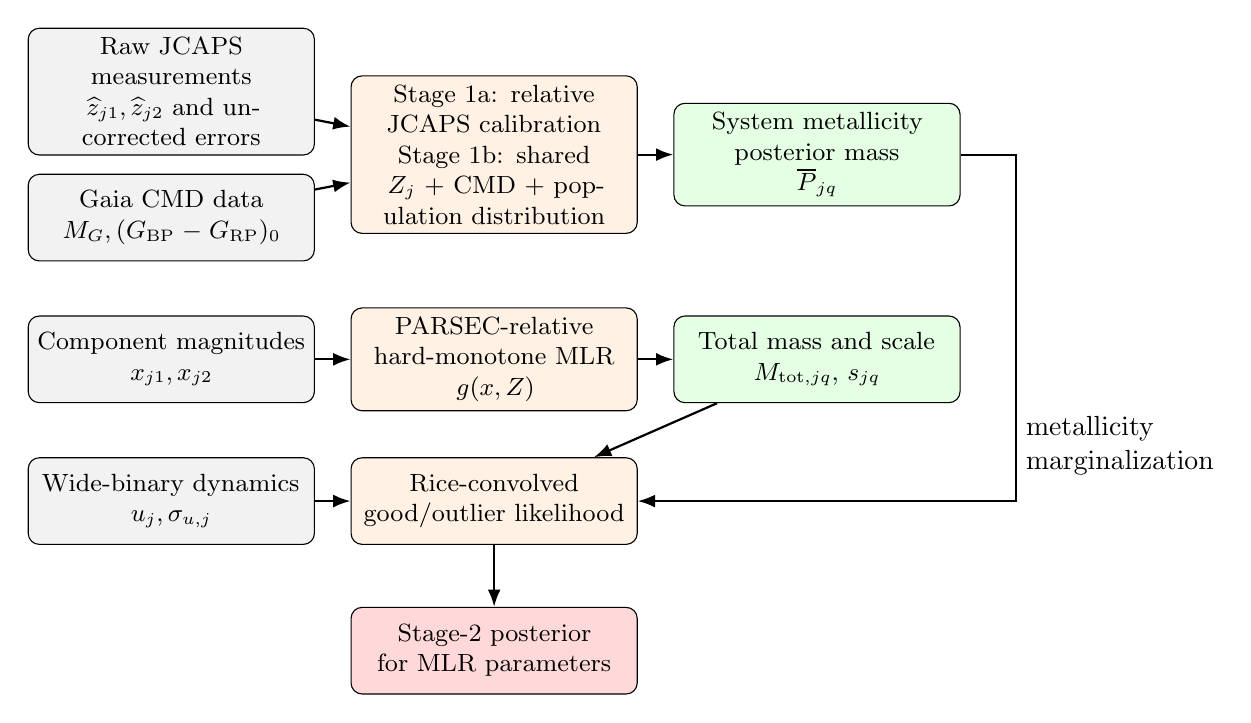
\begin{tikzpicture}[
  box/.style={draw,rounded corners,align=center,minimum height=11mm,
              text width=34mm,fill=blue!5,font=\small},
  data/.style={box,fill=gray!10},
  model/.style={box,fill=orange!10},
  result/.style={box,fill=green!10},
  end/.style={box,fill=red!15},
  arrow/.style={-{Latex[length=2.2mm]},thick},
  cutnote/.style={draw=red!70!black,dashed,rounded corners,
                  text=red!70!black,font=\small\bfseries,
                  fill=white,inner sep=3pt}
]
\node[data]   (spec)   at (0, 2.6) {Raw JCAPS measurements\\$\widehat z_{j1},\widehat z_{j2}$ and uncorrected errors};
\node[data]   (cmd)    at (0, 1.0) {Gaia CMD data\\$M_G,(G_{\rm BP}-G_{\rm RP})_0$};
\node[model]  (stage1) at (4.1, 1.8) {Stage 1a: relative JCAPS calibration\\Stage 1b: shared $Z_j$ + CMD + population distribution};
\node[result] (weights)at (8.2, 1.8) {System metallicity posterior mass\\$\overline P_{jq}$};

\node[data]   (phot)   at (0,-0.8) {Component magnitudes\\$x_{j1},x_{j2}$};
\node[model]  (mlr)    at (4.1,-0.8) {PARSEC-relative\\hard-monotone MLR\\$g(x,Z)$};
\node[result] (mass)   at (8.2,-0.8) {Total mass and scale\\$M_{{\rm tot},jq}$, $s_{jq}$};
\node[data]   (dyn)    at (0,-2.6) {Wide-binary dynamics\\$u_j,\sigma_{u,j}$};
\node[model]  (rice)   at (4.1,-2.6) {Rice-convolved\\good/outlier likelihood};
\node[end] (post)   at (4.1,-4.5) {Stage-2 posterior\\for MLR parameters};

\draw[arrow] (spec) -- (stage1);
\draw[arrow] (cmd) -- (stage1);
\draw[arrow] (stage1) -- (weights);
\draw[arrow] (phot) -- (mlr);
\draw[arrow] (mlr) -- (mass);
\draw[arrow] (mass) -- (rice);
\draw[arrow] (dyn) -- (rice);
\draw[arrow] (rice) -- (post);
\draw[arrow] (weights.east) -- ++(7mm,0) |- node[pos=0.42,right,align=left]
  {metallicity\\marginalization} (rice.east);
% \node[cutnote] at (8.2,0.45) {cut: no dynamical feedback};
\end{tikzpicture}
\caption{Scientific workflow.  Stage~1a estimates the relative JCAPS
calibration from within-binary differences.  Conditional on those fixed
estimates, Stage~1b returns a posterior probability mass over each shared
system metallicity.  Stage~2 propagates this uncertainty into the dynamical MLR
fit but does not update either Stage~1 module.  This one-way flow implements
the modular cut.}
\label{fig:workflow}
\end{figure*}

\section{Observables, latent quantities, and conventions}
\label{sec:notation}

Binary systems are indexed by $j$, their two components by $k\in\{1,2\}$,
and metallicity nodes by $q$.  A hat denotes an observed quantity.  The symbol
$\log_{10}$ is reserved for base-10 stellar-mass logarithms; unqualified
$\log$ denotes the natural logarithm.  ``Dex'' denotes an interval in a
base-10 logarithm.  The main quantities are listed in \cref{tab:notation}.

\begin{table}[htbp]
\centering
\caption{Principal observables and latent or derived quantities.}
\label{tab:notation}
\begin{tabularx}{\textwidth}{@{}lXl@{}}
\toprule
Symbol & Meaning & Unit or range \\
\midrule
$\mathcal D_{\rm 1a}$ & Within-binary JCAPS differences used to estimate $\bm\theta_{\rm rel}$ & data set \\
$\mathcal D_{\rm 1b}$ & JCAPS and Gaia CMD data used for absolute calibration and system posteriors & data set \\
$\mathcal D_{\rm 2}$ & Stage-2 component-magnitude and wide-binary dynamical data, with $\overline P_{jq}$ supplied from Stage~1b & data set \\
$x_{jk}$ & Gaia absolute magnitude of component $k$ & mag \\
$C_{jk}$ & Dereddened colour $(G_{\rm BP}-G_{\rm RP})_0$ & mag \\
$\widehat z_{jk}$ & Raw JCAPS XP metallicity measurement & dex \\
$\sigma_{z,jk}$ & Reported, uncorrected JCAPS uncertainty & dex \\
$Z_j$ & Shared true system metallicity on the PARSEC scale & dex \\
$\overline P_{jq}$ & Stage-1b posterior probability mass at $Z_q$ & $[0,1]$ \\
$g(x,Z)$ & Final $\log_{10}(M/\msun)$ surface & dex \\
$u_j$ & Observed $\Delta v_{\rm tan}\sqrt{r_\perp}$ amplitude & $\kmsau$ \\
$\sigma_{u,j}$ & Component-wise Gaussian error scale entering the Rice model & $\kmsau$ \\
$s_{jq}$ & Dynamical mass scale $\sqrt{M_{{\rm tot},jq}/\msun}$ & dimensionless \\
\bottomrule
\end{tabularx}
\end{table}
\FloatBarrier

The metallicity inputs are strictly
\nolinkurl{feh_jcaps_1}, \nolinkurl{feh_jcaps_2},
\nolinkurl{jc_sigma_m_h_1}, and \nolinkurl{jc_sigma_m_h_2}.
JCAPS infers stellar labels by inverting a forward model of Gaia XP spectra;
the underlying framework and its training strategy are described by
\citet{Li2026JCaPS}.  The names above refer to columns in the analysis table and
are not asserted to be published JCAPS catalogue field names.
No binary-corrected, fitted, calibrated, or inflated metallicity column is used.
Such columns already incorporate the equal-composition assumption that appears
in our likelihood; reusing them would count that information twice and make the
calibration circular.

\section{Stage 1: relative and absolute metallicity calibration}
\label{sec:stage1}

\subsection{Stage 1a: Relative JCAPS calibration}

Before introducing the PARSEC CMD, the relative behavior of JCAPS is calibrated
from the difference between the two stars in each binary.  The adopted
observation model assigns one independent Student-$t$ state to each star,
\begin{equation}
 \widehat z_{jk}\mid Z_j,\delta_z
 \sim \StudentT_{\nu}\!\left[
 Z_j+\delta_z+b_G(x_{jk}),
 \sqrt{\sigma_{z,jk}^2+s_z^2}\right] = \mathcal{L}^{\mathrm{spec}}_{jk}(Z_j),
 \label{eq:spec-model}
\end{equation}
where the second argument is the location and the third is the scale.  The
function $b_G(x)$ is a magnitude-dependent \emph{relative} bias, $s_z$ is one
common additional scale per star (hence a contribution $2s_z^2$ to a binary
difference variance), and $\nu$ is the shared degrees of freedom.  Conditional
on $Z_j$, the two component measurements are independent.  No quality-dependent
mixture state, $\chi^2$-dependent anomaly probability, catastrophic
$-1.5$-dex component, or shared poor-observation offset is included.

More explicitly, let
$d_j=\widehat z_{j1}-\widehat z_{j2}$,
$\Delta b_j=b_G(x_{j1})-b_G(x_{j2})$, and
$a_{jk}=(\sigma_{z,jk}^2+s_z^2)^{1/2}$.  The within-binary difference likelihood is the convolution
\begin{equation}
 p(d_j\mid\Delta b_j,s_z,\nu)=
 \int_{-\infty}^{\infty}
 \StudentT_{\nu}\!\left(e\mid0,a_{j1}\right)
 \StudentT_{\nu}\!\left(e-[d_j-\Delta b_j]\mid0,a_{j2}\right)\dd e.
 \label{eq:difference-convolution}
\end{equation}
The convolution of two Student-$t$ variables is not, in general, another
Student-$t$ distribution.  Both $Z_j$ and the common offset $\delta_z$ cancel
from $d_j$, but the observed differences still constrain the relative-bias
shape $b_G$, the per-star excess scale $s_z$, and the common tail parameter
$\nu$.  Stage~1a obtains the maximum-likelihood estimate
\begin{equation}
 \widehat{\bm\theta}_{\rm rel}
 =\arg\max_{\bm\theta_{\rm rel}}\sum_{j\in\mathcal D_{\rm 1a}}
 \log p(d_j\mid\bm\theta_{\rm rel}),
 \qquad \bm\theta_{\rm rel}=(b_G,s_z,\nu),
 \label{eq:relative-mle}
\end{equation}
and checks the resulting difference distribution on a held-out subset that is
not used in this maximization.  The differences cannot determine an absolute
metallicity zero point.  We set
$b_G(8.5)=0$ and use the frozen
plug-in values
\begin{align}
 x_{\rm knot}/{\rm mag} &= (3.5,6.0,8.5,11.0,13.5),\\
 b_G(x_{\rm knot})/{\rm dex} &= (0.11,0.05,0,
 -0.31,-0.53),\\
 s_z &=0.05\ {\rm dex},\qquad \nu=2.5,
\end{align}
with linear interpolation between knots.  Stage~1b conditions on
$\widehat{\bm\theta}_{\rm rel}$: these three quantities are fixed inputs, not
parameters assigned priors or re-estimated in Stage~1b.

\subsection{Stage 1b: Absolute calibration and system metallicity posteriors}

\subsubsection{Hierarchical population distribution}

The latent metallicities of the selected systems follow
\begin{equation}
 p_{\rm pop}(Z\mid\bm\omega)=\sum_{r=1}^{6}\omega_r
 \varphi_r^{\rm trunc}(Z),\qquad
 \bm\omega\sim\operatorname{Dirichlet}(1,\ldots,1),
 \label{eq:pop}
\end{equation}
where every $\varphi_r^{\rm trunc}$ is a Gaussian density renormalized on
$-1.0\le Z\le0.6$ dex.  Writing $\phi$ and $\Phi$ for the standard-normal
density and cumulative distribution function, respectively,
\begin{equation}
 \varphi_r^{\rm trunc}(Z)=
 \frac{\phi[(Z-\mu_r)/\tau_r]}
 {\tau_r\!\left\{\Phi[(Z_{\max}-\mu_r)/\tau_r]
 -\Phi[(Z_{\min}-\mu_r)/\tau_r]\right\}}
 \indicator(Z_{\min}\le Z\le Z_{\max}).
 \label{eq:truncated-gaussian-basis}
\end{equation}
Here $Z_{\min}=-1.0$ and $Z_{\max}=0.6$ dex, the six centers $\mu_r$ are
equally spaced between these limits, and every $\tau_r=1.6/6=0.2667$ dex.
This hierarchical population distribution is learned jointly with the other
Stage-1b parameters; it is not an independently estimated external prior.
Because it describes the systems after sample selection, it must not be
interpreted as the intrinsic Galactic metallicity distribution function.

The remaining common offset is assigned
\begin{equation}
 \delta_z\sim\Normal(0,0.3^2)\quad\text{dex}.
 \label{eq:delta-prior}
\end{equation}
Under the sign convention of \cref{eq:spec-model}, positive $\delta_z$ means
that JCAPS measurements lie above the PARSEC metallicity scale at fixed $Z_j$.

\subsubsection{PARSEC CMD likelihood and the 4000-K mask}

The PARSEC surface supplies predicted colour $C_{\rm P}(x,Z)$ and effective
temperature $T_{\rm eff,P}(x,Z)$ \citep{Bressan2012PARSEC}.  The repository
records the age, metallicity, and magnitude coverage of the local PARSEC table,
but not enough provenance to identify a more specific PARSEC release or Gaia
passband realization; we therefore make no more specific version claim.  The
formal colour uncertainty is propagated
from the BP and RP signal-to-noise ratios,
\begin{equation}
 \sigma_{C,jk}=\frac{2.5}{\ln 10}
 \left(\mathrm{SNR}_{\rm BP,jk}^{-2}
 +\mathrm{SNR}_{\rm RP,jk}^{-2}\right)^{1/2}.
\end{equation}
For an eligible component, the CMD likelihood is
\begin{equation}
 C_{jk} \mid Z_j \sim \StudentT_{4}\!\left[
 C_{\rm P}(x_{jk},Z_j),
 \sqrt{\sigma_{C,jk}^2+s_C^2}\right] =  \mathcal{L}^{\rm CMD}_{jk}(Z_j).
 \label{eq:cmd}
\end{equation}
The colour zero point is fixed to zero and
$s_C\sim\operatorname{HalfNormal}(0.1\ {\rm mag})$.  To avoid allowing membership in the
CMD term to change with a proposed metallicity, eligibility is fixed over the
full latent-metallicity domain:
\begin{equation}
 m_{jk}=\indicator\!\left[
 \min_{q\in\mathcal Q}T_{\rm eff,P}(x_{jk},Z_q)\ge4000\ {\rm K}\right].
 \label{eq:warm-mask}
\end{equation}
If $m_{jk}=0$, that star still contributes its JCAPS likelihood but not its CMD
likelihood.  To construct the fixed CMD reference surface, we selected PARSEC
rows with $9.3<\log_{10}(\mathrm{age/yr})<10.0$ and
$3<G_{\rm mag}<15$.  At fixed source-table $G_{\rm mag}$ and metallicity, rows
from the selected ages were averaged separately in colour and
$\log T_{\rm eff}$, so age is not a latent variable in this analysis.  Colour
was represented by an up-to-cubic smoothing spline with smoothing parameter
$0.001$; $\log T_{\rm eff}$ was linearly interpolated and then exponentiated
before tabulation.  The colour and linear-$T_{\rm eff}$ tables were evaluated
bilinearly in $(M_G,Z)$ on a 500-point magnitude grid spanning
$3.5\le M_G\le13.5$.  This CMD construction is distinct from the
$501\times81$ $(M_G,Z)$ grid used only to fit the MLR's fixed PARSEC mass
projection.

The frozen sample contains 14,876 binaries (29,752 stars).  The 4000-K rule
admits 12,167 stars; 8,247 systems have at least one eligible component and
3,920 have two.  These counts describe CMD coverage, not evidence that the
cool-star PARSEC colours are correct.

\subsubsection{System posterior and the cut object}

The sampled Stage-1b global parameters are exactly
$\bm\psi=(\delta_z,s_C,\bm\omega)$.  Conditional on
$\widehat{\bm\theta}_{\rm rel}$, the unnormalized metallicity density for one
system is
\begin{equation}
 \widetilde p_j(Z\mid\bm\psi,\widehat{\bm\theta}_{\rm rel})
 =p_{\rm pop}(Z\mid\bm\omega)
 \prod_{k=1}^{2}\mathcal{L}^{\rm spec}_{jk}
 (Z\mid\delta_z,\widehat{\bm\theta}_{\rm rel})
 \left[\mathcal{L}^{\rm CMD}_{jk}(Z\mid s_C)\right]^{m_{jk}}.
 \label{eq:zpost-cont}
\end{equation}
The global parameters are inferred from the product of the system-level
marginal evidences, rather than from separately normalized system posteriors:
\begin{equation}
 p(\bm\psi\mid\mathcal D_{\rm 1b},\widehat{\bm\theta}_{\rm rel})\propto
 p(\delta_z)\,p(s_C)\,p(\bm\omega)
 \prod_j\left[\sum_{q\in\mathcal Q}w_q^{(Z)}
 \widetilde p_j(Z_q\mid\bm\psi,\widehat{\bm\theta}_{\rm rel})\right].
 \label{eq:stage1-global}
\end{equation}
The model evaluates this expression at 81 equally spaced nodes
$Z_q\in[-1.0,0.6]$ dex using trapezoidal integration weights $w_q^{(Z)}$:
\begin{equation}
 P_{jq}(\bm\psi,\widehat{\bm\theta}_{\rm rel})=
 \frac{w_q^{(Z)}\widetilde p_j
 (Z_q\mid\bm\psi,\widehat{\bm\theta}_{\rm rel})}
 {\sum_{q'}w_{q'}^{(Z)}\widetilde p_j
 (Z_{q'}\mid\bm\psi,\widehat{\bm\theta}_{\rm rel})}.
\end{equation}
The saved quantity passed to Stage~2 is the posterior average
\begin{equation}
 \overline P_{jq}=\mathbb E_{\bm\psi\mid\mathcal D_{\rm 1b},
 \widehat{\bm\theta}_{\rm rel}}
 \left[P_{jq}(\bm\psi,\widehat{\bm\theta}_{\rm rel})\right].
 \label{eq:pbar}
\end{equation}
Each system helps learn the shared hyperparameters $\bm\psi$ and is then
partially pooled through their hyperposterior.  This standard hierarchical
self-influence is not likelihood double-counting: each observation enters the
joint Stage-1b likelihood once.  The average in \cref{eq:pbar} integrates over
the global hyperposterior rather than plugging in a single value of
$\bm\psi$.  Thus Stage~2 receives a probability distribution rather than a
metallicity point estimate.  Because $\overline P_{jq}$ already includes
$p_{\rm pop}$, both spectroscopic likelihoods, every eligible CMD likelihood,
and the metallicity quadrature weights, Stage~2 must not multiply any of these
population or quadrature factors again.

\section{Stage 2: a PARSEC-relative hard-monotone MLR}
\label{sec:mlr}

\subsection{Baseline projection and scientific correction}

Let the original PARSEC mass surface be
\begin{equation}
 g_{\rm P}(x,Z)=\log_{10}\!\left[\frac{M_{\rm P}(x,Z)}{\msun}\right].
\end{equation}
The finite MLR basis cannot reproduce this tabulated surface exactly.  The projected PARSEC mass surface onto the same tensor-product B-spline basis used by the fitted model is represented as $g_{\rm P}^{*}(x,Z)$, 
\begin{equation}
 g_{\rm P}^{*}(x,Z)=\sum_{i=1}^{K_x}\sum_{h=1}^{K_Z}
 \Pi_{ih}B_i(x)C_h(Z),
\end{equation}
where $\Pi$ is fixed.  The fitted correction is
\begin{equation}
 \Delta_*(x,Z)=\sum_{i,h}D_{ih}B_i(x)C_h(Z),
 \qquad \Theta_{ih}=\Pi_{ih}+D_{ih},
\end{equation}
and hence the fitted mass surface is
\begin{equation}
 g(x,Z)=\sum_{i,h}\Theta_{ih}B_i(x)C_h(Z)
       =g_{\rm P}^{*}(x,Z)+\Delta_*(x,Z).
 \label{eq:g-total}
\end{equation}
The quantity reported scientifically relative to the original PARSEC table is
not $\Delta_*$ alone but
\begin{equation}
 \Delta_{\rm P}(x,Z)=g(x,Z)-g_{\rm P}(x,Z)
 =\Delta_*(x,Z)+\epsilon_{\rm P}(x,Z),
 \quad \epsilon_{\rm P}=g_{\rm P}^{*}-g_{\rm P}.
 \label{eq:delta-parsec}
\end{equation}
where $\epsilon_{\rm P}$ is the deterministic projection error, the RMS and maximum absolute values of
$\epsilon_{\rm P}$ are 0.002 and 0.019 dex, respectively.

The adopted basis has $K_x\times K_Z=8\times4$ cubic B-splines
\citep{deBoor2001Splines}.  Both knot vectors are open and clamped:
\begin{align}
 \bm\kappa_x={}&(3.5,3.5,3.5,3.5,5.5,7.5,9.5,11.5,
                  13.5,13.5,13.5,13.5)\ {\rm mag},\\
 \bm\kappa_Z={}&(-1.0,-1.0,-1.0,-1.0,0.6,0.6,0.6,0.6)\ {\rm dex}.
\end{align}

\subsection{Hard monotonicity of the total mass surface}

At fixed metallicity, increasing $M_G$ means a fainter star and must not
increase its mass.  At fixed magnitude, the adopted physical assumption is
that increasing metallicity must not decrease the mass.  We therefore require
\begin{equation}
 \Theta_{i+1,h}\le\Theta_{ih},\qquad
 \Theta_{i,h+1}\ge\Theta_{ih}.
 \label{eq:coefficient-order}
\end{equation}
Because B-spline derivatives are non-negative lower-degree basis functions
weighted by adjacent control-coefficient differences, these inequalities imply
throughout the continuous domain
\begin{equation}
 \frac{\partial g}{\partial x}\le0,
 \qquad \frac{\partial g}{\partial Z}\ge0.
\end{equation}
The constraints apply to the \emph{total} coefficient surface $\Theta=\Pi+D$,
not to the correction $D$ alone.  The correction is consequently free to
increase or decrease in either coordinate.  We also impose no sign constraint
on its mixed differences; doing so would add an unsupported assumption about
how the magnitude slope changes with metallicity.  The constructive
parameterization that enforces \cref{eq:coefficient-order} is given in
\cref{app:monotone}.

% \subsection{Shrinkage, smoothness, and the solar anchor}

% The difference $D=\Theta-\Pi$ is deterministic and does not receive a second
% set of independent coefficient priors.  Instead, PARSEC-relative shrinkage is
% expressed by
% \begin{equation}
%  \log\pi_{\rm shrink}(D)=-\frac{1}{2\tau_D^2}\sum_{i,h}D_{ih}^2+\mathrm{const},
%  \qquad \tau_D=0.10\ {\rm dex}.
% \end{equation}
% Separate quadratic potentials regularize the spacing-aware second differences
% in $x$ and $Z$ and the mixed difference, following the general use of
% coefficient-difference penalties for B-spline smoothing
% \citep{EilersMarx1996PSplines}, with
% $\tau_x=\tau_Z=\tau_{xZ}=0.05$ dex.  Let $\xi_i^x$ and $\xi_h^Z$ be the
% Greville abscissae, $h_i^x=\xi_{i+1}^x-\xi_i^x$ and
% $h_h^Z=\xi_{h+1}^Z-\xi_h^Z$, and let
% $\bar h_x=(\xi_{K_x}^x-\xi_1^x)/(K_x-1)$ and
% $\bar h_Z=(\xi_{K_Z}^Z-\xi_1^Z)/(K_Z-1)$.  The implemented differences are
% \begin{align}
%  D^{(2,x)}_{ih}&=
%  \frac{2\bar h_x^2}{h_i^x+h_{i+1}^x}
%  \left[\frac{D_{i+2,h}-D_{i+1,h}}{h_{i+1}^x}
%        -\frac{D_{i+1,h}-D_{i,h}}{h_i^x}\right],\\
%  D^{(2,Z)}_{ih}&=
%  \frac{2\bar h_Z^2}{h_h^Z+h_{h+1}^Z}
%  \left[\frac{D_{i,h+2}-D_{i,h+1}}{h_{h+1}^Z}
%        -\frac{D_{i,h+1}-D_{i,h}}{h_h^Z}\right],\\
%  D^{(xZ)}_{ih}&=
%  \frac{\bar h_x\bar h_Z}{h_i^x h_h^Z}
%  \left(D_{i+1,h+1}-D_{i+1,h}-D_{i,h+1}+D_{i,h}\right).
% \end{align}
% Their contribution is
% \begin{equation}
%  \log\pi_{\rm smooth}(D)=-\frac12\sum_{i,h}
%  \left(\frac{D^{(2,x)}_{ih}}{\tau_x}\right)^2
%  -\frac12\sum_{i,h}\left(\frac{D^{(2,Z)}_{ih}}{\tau_Z}\right)^2
%  -\frac12\sum_{i,h}\left(\frac{D^{(xZ)}_{ih}}{\tau_{xZ}}\right)^2
%  +\mathrm{const}.
% \end{equation}
% The sums cover only indices for which the relevant neighbors exist.  The
% spacing normalization retains the dex scale of the stated hyperparameters.
% These terms favor a small, smooth correction; they do not enforce the signs of
% slopes or curvature.

% The absolute mass scale is weakly anchored at the solar reference point:
% \begin{equation}
%  g(4.67,0)\sim\Normal\!\left(0,
%  \left[\frac{0.01}{\ln10}\right]^2\right).
%  \label{eq:solar}
% \end{equation}
% This is a 1\% mass-scale constraint expressed in dex.  It constrains the final
% surface rather than forcing $\Delta_{\rm P}(4.67,0)=0$.  It is a soft Gaussian
% anchor, not an exact equality, so posterior surfaces need not pass exactly
% through zero log mass at the solar reference point.

\section{Wide-binary dynamical likelihood}
\label{sec:dynamics}

\subsection{Mass-scaled velocity statistic}

In binary orbital motion, the system mass ($m_{\mathrm{tot}} = m_1+m_2$), component separation ($a$), true anomaly $\theta$ and eccentricity $e$ set the instantaneous relative speed,
\begin{equation}
    v_{\rm rel} = \sqrt{\frac{G\,(m_1+m_2)}{a}}\; f(\theta,e),
\end{equation}
with $f(\theta,e)$ encapsulating the phase dependence along the ellipse. At pericenter ($\theta=0$),
\begin{equation}
    v_{\rm rel,peri} = \sqrt{\frac{G\,(m_1+m_2)}{a}} \sqrt{\frac{1+e}{1-e}},
\end{equation}
and at apocenter ($\theta=\pi$),
\begin{equation}
    v_{\rm rel,apo} = \sqrt{\frac{G\,(m_1+m_2)}{a}} \sqrt{\frac{1-e}{1+e}}.
\end{equation}

To connect physics with observables we define
\begin{equation}
    u := v \sqrt{s},
\end{equation}
where $v$ is the projected relative speed and $s$ is the projected separation. Under this definition, $u \propto \sqrt{m_{\rm tot}/\msun}$ and depends on nuisance parameters $\theta$, $e$, and orientation $\phi$. We again separate the mass dependence by defining $\tilde{u} \equiv u/\sqrt{m_{\rm tot}/\msun}$, so $\tilde{u}$ depends only on the nuisance parameters and their influence can be marginalized. We perform simulations and pre-fit $p(\tilde{u})$ by integrating $p(\tilde{u}\,|\,\phi,\theta,e)$ over the nuisance distributions. For an observed $u$ the likelihood then becomes
\begin{equation}
    p(u\,|\,m_{\rm tot}) = \frac{1}{\sqrt{m_{\rm tot}/\msun}}\,p\!\left(\tilde{u} \equiv \frac{u}{\sqrt{m_{\rm tot}/\msun}}\right).
\end{equation}

Our goal is to constrain the mass--luminosity mapping $\mathcal{M}$, which links photometric observables to stellar mass. We treat
\begin{equation}
    \{M_{\rm G}, {\rm BP-RP}, Z\} = \mathcal{M}(m,\,Z),
\end{equation}
with parameters $\Theta$ defining the functional form.  Conversely, stellar
masses are obtained from the inverse map
$m=\mathcal{M}^{-1}(M_{\rm G},Z;\Theta)$. The likelihood for one measurement is then

\begin{align}
    &\mathcal{L}_j \\
    &\quad = p \left(u_j \big|\ m_{\rm tot};\mathcal{M}^{-1}(M_{{\rm G},j1}, Z_j;\Theta) + \mathcal{M}^{-1}(M_{{\rm G},j2},Z_j;\Theta) \right). \notag
\end{align}

Measurement uncertainties on the tangential velocity enter mainly through the uncertainty of the proper-motion difference $\Delta\mu$ in the relation of 
\begin{equation}
    u = 4.74 \times \frac{\Delta\mu}{\varpi} \times \sqrt{s}.
\end{equation}
Assuming Rice-distributed proper-motion differences,
\begin{align}
    &\mathrm{Rice}(\Delta\mu_{\rm obs}\,|\,\Delta\mu_{\rm true},\sigma_{\Delta\mu}) = \frac{\Delta\mu_{\rm obs}}{\sigma_{\Delta\mu}^2} \notag\\
    &\quad \times \exp\!\left[-\frac{\Delta\mu_{\rm obs}^2 + \Delta\mu_{\rm true}^2}{2\sigma_{\Delta\mu}^2}\right] I_0\!\left(\frac{\Delta\mu_{\rm obs}\,\Delta\mu_{\rm true}}{\sigma_{\Delta\mu}^2}\right),
\end{align}
the distribution for $u$ is
\begin{align}
    &\mathrm{Rice}(u_j\,|\,u_{\rm true},\sigma_{u,j}) = \frac{u_j}{\sigma_{u,j}^2}  \notag\\
    \quad &\times \exp\!\left[-\frac{u_j^2 + u_{\rm true}^2}{2\sigma_{u,j}^2}\right] I_0\!\left(\frac{u_j\,u_{\rm true}}{\sigma_{u,j}^2}\right),
\end{align}
where $I_0$ is the zeroth-order modified Bessel function. Integrating over $\tilde{u}$ yields
\begin{align}
    &p(u_j\,|\,m_{\rm tot}) \\
    &= \frac{1}{\sqrt{m_{\rm tot}/\msun}} \int_0^\infty \mathrm{Rice}\!\left(\frac{u_j}{\sqrt{m_{\rm tot}/\msun}} \,\bigg|\, \tilde{u}, \frac{\sigma_{u,j}}{\sqrt{m_{\rm tot}/\msun}}\right) p(\tilde{u})\, d\tilde{u}. \notag
\end{align}

To allow for outliers we adopt a mixture model for each datum,

\begin{equation}
\begin{aligned}
    \mathcal{L}^{\rm mix}_j = \int~ \Biggl[ & (1-f_{\mathrm{outlier}}) \cdot \dfrac{1}{\sqrt{m_{\mathrm{tot}}/\msun}} \cdot p\left( \tilde{u} \right) \\
    & + f_{\mathrm{outlier}} \cdot \dfrac{1}{\sqrt{m_{\mathrm{tot}}/\msun}} \cdot \dfrac{1}{C_{\mathrm{o}}} \cdot G_{\mathrm{o}}\left( \tilde{u}|\mu_{\mathrm{o}},~\sigma^2_{\mathrm{o}} \right) \Biggr] \\
    & \times \mathrm{Rice} \left(\dfrac{u_{\mathrm{obs}}}{\sqrt{m_{\mathrm{tot}}/\msun}}|\tilde{u},\dfrac{\sigma_{u,j}}{\sqrt{m_{\mathrm{tot}}/\msun}}\right) ~d\tilde{u}.
\end{aligned}
\end{equation}


The mass-luminosity relation can thus be constrained by substituting $m_{\mathrm{tot}}$ with

\begin{align}
    m_{\mathrm{tot}} = \mathcal{M}^{-1}(M_{\mathrm{G},1},Z;\Theta) + \mathcal{M}^{-1}(M_{\mathrm{G},2},Z;\Theta)
\end{align}

% At metallicity node $Z_q$, the component and total masses predicted by the MLR
% are
% \begin{equation}
%  M_{jkq}=\msun 10^{g(x_{jk},Z_q)},\qquad
%  M_{{\rm tot},jq}=M_{j1q}+M_{j2q},
% \end{equation}
% and the scale acting on the normalized velocity distribution is
% \begin{equation}
%  s_{jq}=\sqrt{M_{{\rm tot},jq}/\msun}.
%  \label{eq:mass-scale}
% \end{equation}
% Following the mass-scaled wide-binary statistic used by
% \citet{Hwang2024DynamicalMasses}, the observed quantity is
% \begin{equation}
%  u_j=\Delta v_{{\rm tan},j}\sqrt{r_{\perp,j}},
%  \label{eq:u}
% \end{equation}
% in $\kmsau$.  When constructed from proper motion, parallax, and projected
% separation, its numerical form is
% \begin{equation}
%  u_j=4.74\,\frac{\Delta\mu_j}{\varpi_j}
%  \sqrt{r_{\perp,j}/{\rm AU}},
% \end{equation}
% with consistent angular units for $\Delta\mu_j$ and $\varpi_j$.  The reported
% dynamical uncertainty is represented by $\sigma_{u,j}$; when the input reports
% the significance of the proper-motion difference, it is constructed as
% $\sigma_{u,j}=u_j/(\mathrm{dpm/error})_j$.

% \subsection{Rice measurement model and latent velocity distribution}

% The measured quantity is the magnitude of a two-dimensional velocity
% difference.  If the two Cartesian measurement errors are independent Gaussians
% with common scale $\sigma$, the conditional amplitude density is the Rice
% distribution \citep{Rice1945},
% \begin{equation}
%  R(u\mid v,\sigma)=\frac{u}{\sigma^2}
%  \exp\!\left[-\frac{u^2+v^2}{2\sigma^2}\right]
%  I_0\!\left(\frac{uv}{\sigma^2}\right),\qquad u\ge0,
%  \label{eq:rice}
% \end{equation}
% where $v$ is the latent true amplitude and $I_0$ is the modified Bessel
% function.  Unlike an untruncated one-dimensional Gaussian, this likelihood
% respects the non-negative amplitude and remains appropriate near zero.

% Let $\widetilde u$ denote the latent statistic after removing the mass scale,
% so that $v=s\widetilde u$.  For component $c\in\{\mathrm{good,out}\}$,
% \begin{equation}
%  L_{c,j}(s)=\int_{\mathcal U_c}
%  R(u_j \mid s\widetilde u,\sigma_{u,j})
%  p_c(\widetilde u)\dd\widetilde u.
%  \label{eq:component-like}
% \end{equation}
% Equivalently, integration over $v$ gives
% \begin{equation}
%  L_{c,j}(s)=\int_{s\mathcal U_c}
%  R(u_j \mid v,\sigma_{u,j})
%  p_c(v/s)\frac{\dd v}{s};
%  \label{eq:jacobian}
% \end{equation}
% the Jacobian $1/s$ is essential.

% The functional form of the good-component basis follows
% \citet{Hwang2024DynamicalMasses}:
% \begin{equation}
%  p_{\rm good}(\widetilde u)=A\widetilde u
%  \exp\!\left[-B\widetilde u^2-
%  \exp\!\left(\frac{\widetilde u-u_c}{C}\right)\right]
%  \indicator(0<\widetilde u\le80),
%  \label{eq:good}
% \end{equation}
% with $A=5.434\times10^{-3}$, $B=2.544\times10^{-3}$,
% $u_c=35.67$, and $C=3.100$ in the units implied by $\widetilde u$.
% These numerical constants are frozen project-specific choices whose derivation
% is not documented.  They are not the
% constants reported by \citet{Hwang2024DynamicalMasses}, who give
% $A=4.95\times10^{-3}$, $B=2.24\times10^{-3}$, $u_0=36.09$, and $C=3.85$ for
% their fitted distribution.  We therefore cite that work for the normalized
% statistic and functional form, but not as the source of the frozen constants.
% Its area on $[0,80]$ is 0.9978600946, not exactly unity.  The outlier component
% is a Gaussian with mean 40 and standard deviation 13, truncated and normalized
% on $[0,80]$.  These outlier constants are also frozen project choices rather
% than values attributed to an external publication:
% \begin{equation}
%  p_{\rm out}(\widetilde u)=
%  \frac{\phi[(\widetilde u-40)/13]}
%  {13\{\Phi[(80-40)/13]-\Phi(-40/13)\}}
%  \indicator(0\le\widetilde u\le80).
%  \label{eq:out}
% \end{equation}
% The component shapes are fixed.  Their mixture is
% \begin{equation}
%  L_j^{\rm mix}(s)=(1-f_{\rm outlier})L_{{\rm good},j}(s)
%  +f_{\rm outlier}L_{{\rm out},j}(s),
%  \qquad f_{\rm outlier}\sim\operatorname{Beta}(3,12).
%  \label{eq:mixture}
% \end{equation}
% Because \cref{eq:good} retains its raw, slightly non-normalized amplitude,
% $f_{\rm outlier}$ is an effective likelihood weight and cannot be interpreted as
% the physical fraction of outlier binaries.

\subsection{Metallicity marginalization}

At metallicity node $Z_q$, the component masses, total mass, and dynamical
mass scale are
\begin{equation}
 m_{jkq}=\mathcal{M}^{-1}(M_{{\rm G},jk},Z_q;\Theta),\qquad
 M_{{\rm tot},jq}=m_{j1q}+m_{j2q},\qquad
 s_{jq}=\sqrt{M_{{\rm tot},jq}/\msun}.
 \label{eq:node-mass-scale}
\end{equation}

For one system, the final Stage-2 likelihood is
\begin{equation}
 \mathcal L_j^{\rm dyn}(\bm\theta_M)=
 \sum_{q=1}^{81}\overline P_{jq}
 \mathcal L_j^{\rm mix}\!\left[s_{jq}(\bm\theta_M)\right].
 \label{eq:dyn-final}
\end{equation}
This sum propagates the system's Stage-1b metallicity uncertainty into its mass
and dynamics.  It is not a second use of the spectroscopic or CMD data.
Population-distribution factors and additional quadrature weights must not be
inserted in \cref{eq:dyn-final}, because both are already present in the
probability masses $\overline P_{jq}$.

\section{Parameters, priors, and posterior computation}
\label{sec:inference}

The sampled MLR coordinates are
\begin{equation}
 \bm\theta_M=\left(c_0,\{a_h\}_{h=2}^{K_Z},
 \{b_i\}_{i=2}^{K_x},\{r_{ih}\}_{i,h\ge2},
 \log\lambda_x,\log\lambda_Z,f_{\rm outlier}\right),
\end{equation}
giving 35 scalar degrees of freedom for $K_x=8$ and $K_Z=4$.  The priors and
fixed regularization scales are summarized in \cref{tab:priors}.  Here
$\Pi_{11}=0.00703$, and the PARSEC-derived reference increments are
$\lambda_{x,\rm ref}=0.18624$ and $\lambda_{Z,\rm ref}=0.13078$ dex.

\begin{table}[htbp]
\centering
\caption{Frozen Stage-1a, Stage-1b, and Stage-2 parameter specification.  Normal
distributions are written as location and standard deviation.}
\label{tab:priors}
\begin{tabularx}{\textwidth}{@{}lllX@{}}
\toprule
Stage & Quantity & Prior or fixed value & Role \\
\midrule
1a & $\bm\theta_{\rm rel}$ & MLE; no prior & Difference calibration $(b_G,s_z,\nu)$; fixed in Stage~1b \\
1b & $\delta_z$ & $\Normal(0,0.3)$ dex & JCAPS--PARSEC zero point \\
1b & $s_C$ & Half-Normal$(0.1)$ mag & CMD excess colour scatter \\
1b & $\bm\omega$ & Dirichlet$(1,\ldots,1)$ & Six-component population weights \\
\addlinespace
2 & $c_0$ & $\Normal(\Pi_{11},0.10)$ dex & First total-surface coefficient \\
2 & $a_h,b_i,r_{ih}$ & $\Normal(0,1)$ & Unconstrained monotone coordinates \\
2 & $\log\lambda_x$ & $\Normal(\log0.18624,0.7)$ & Magnitude increment scale \\
2 & $\log\lambda_Z$ & $\Normal(\log0.13078,0.7)$ & Metallicity increment scale \\
2 & $f_{\rm outlier}$ & Beta$(3,12)$ & Effective component weight \\
% 2 & $\tau_D$ & 0.10 dex & PARSEC-relative shrinkage \\
% 2 & $\tau_x,\tau_Z,\tau_{xZ}$ & 0.05 dex each & Spacing-aware smoothness potentials \\
% 2 & solar anchor & $g(4.67,0)=0\pm0.01/\ln10$ dex & Absolute mass scale \\
\bottomrule
\end{tabularx}
\end{table}
\FloatBarrier

Stage~1b and Stage~2 were sampled with the No-U-Turn Sampler (NUTS)
\citep{HoffmanGelman2014NUTS}, using four chains and 1,000 retained draws per
chain.  The frozen fits had no divergent transitions.  Posterior adequacy must
additionally be assessed with rank-based
$\widehat R$, effective sample sizes, chain traces, and posterior predictive or
held-out checks; successful execution alone is not scientific validation.

\section{Information propagated, assumptions, and limitations}
\label{sec:limitations}

\Cref{tab:uncertainties} distinguishes uncertainty that is represented in the
current likelihood from uncertainty held fixed or omitted.  In particular, the
model propagates the reported per-star JCAPS errors, heavy-tailed metallicity
scatter, CMD colour scatter, the single-system metallicity posterior, and the
reported dynamical amplitude error.  It does not propagate uncertainty in the
absolute magnitudes, extinction correction, PARSEC model family, age
distribution, or uncertainty in the preliminary Stage-1a relative-calibration
estimates.

\begin{table}[htbp]
\centering
\caption{Uncertainty and information flow in the frozen model.}
\label{tab:uncertainties}
\begin{tabularx}{\textwidth}{@{}lXX@{}}
\toprule
Category & Represented & Not represented or deliberately cut \\
\midrule
Metallicity & Raw per-star errors, shared $Z_j$, Student-$t$ tails,
CMD excess scatter, population weights, and each system's $\overline P_{jq}$
& Uncertainty in the fixed preliminary Stage-1a estimates $b_G$, $s_z$, and
$\nu$; cross-system covariance induced by shared Stage-1b parameters \\
Photometry and models & Formal BP/RP colour errors and fitted $s_C$
& $M_G$ uncertainty, extinction uncertainty, age as a latent variable,
PARSEC-family/model discrepancy \\
Dynamics & Rice convolution with reported $\sigma_{u,j}$ and latent velocity
component distributions & Uncertainty in the fixed good/outlier shapes and
additional astrometric covariance beyond the reported $\sigma_{u,j}$ \\
Feedback & Metallicity uncertainty is passed from Stage~1b to Stage~2
& Dynamics cannot update $\delta_z$, $s_C$, $\bm\omega$, or individual
metallicity posteriors \\
\bottomrule
\end{tabularx}
\end{table}

\FloatBarrier
Several interpretation boundaries follow.  First, the shared $Z_j$ is a model
assumption for a co-natal binary, not direct proof that both stars have identical
surface abundances.  Second, the 4000-K threshold expands CMD coverage but may
also increase sensitivity to low-temperature PARSEC colour systematics.  Third,
hard monotonicity encodes the adopted physical ordering of the MLR; it does not
demonstrate that PARSEC or the observations are unbiased over the full domain.
Fourth, the cut reduces feedback from a potentially misspecified dynamical
model, but it understates joint uncertainty by fixing the Stage-1a estimates,
discarding the shared Stage-1b posterior covariance, and excluding any
information that the dynamics could provide about metallicity calibration.  A
fully joint analysis would be a different model,
not merely a more accurate implementation of the present one.

\appendix
\section{Constructive monotone reparameterization}
\label{app:monotone}

The total coefficient grid $\Theta$ is generated from unconstrained raw
variables rather than by rejecting proposals that violate inequalities.  Define
$\softplus(t)=\log(1+e^t)$ and
$\sigmoid(t)=(1+e^{-t})^{-1}$.  With positive scales
$\lambda_x=e^{\log\lambda_x}$ and $\lambda_Z=e^{\log\lambda_Z}$, construct the
first row and column as
\begin{align}
 \Theta_{11}&=c_0,\\
 \Theta_{1h}&=\Theta_{1,h-1}+\lambda_Z\softplus(a_h),
 &&h=2,\ldots,K_Z,\\
 \Theta_{i1}&=\Theta_{i-1,1}-\lambda_x\softplus(b_i),
 &&i=2,\ldots,K_x.
 \label{eq:boundaries}
\end{align}
The first row therefore increases with $Z$, whereas the first column decreases
with $x$.  Interior points are visited in increasing $i+h$.  For each point,
define
\begin{equation}
 L_{ih}=\Theta_{i,h-1},\qquad U_{ih}=\Theta_{i-1,h},
\end{equation}
and set
\begin{equation}
 \Theta_{ih}=L_{ih}+(U_{ih}-L_{ih})\sigmoid(r_{ih}),
 \qquad i,h\ge2.
 \label{eq:interior}
\end{equation}
If all previously constructed points obey the two monotone orders, then
\begin{equation}
 L_{ih}=\Theta_{i,h-1}\le\Theta_{i-1,h-1}\le
 \Theta_{i-1,h}=U_{ih}.
\end{equation}
Thus \cref{eq:interior} lies inside a non-empty interval and simultaneously
satisfies
$\Theta_{i,h-1}\le\Theta_{ih}\le\Theta_{i-1,h}$.  Induction over $i+h$
therefore proves the coefficient inequalities in \cref{eq:coefficient-order}
for the complete grid.  Finally, $D=\Theta-\Pi$ is computed deterministically.

For completeness, the derivative identity for a degree-$d_x$ B-spline surface
has the form
\begin{equation}
 \frac{\partial g}{\partial x}=
 \sum_{i=1}^{K_x-1}\sum_{h=1}^{K_Z}
 \rho_{x,i}(\Theta_{i+1,h}-\Theta_{ih})
 \widetilde B_i(x)C_h(Z),\qquad \rho_{x,i}>0,
\end{equation}
where $\widetilde B_i$ is a non-negative degree-$(d_x-1)$ basis function.
The corresponding $Z$ derivative contains
$\rho_{Z,h}(\Theta_{i,h+1}-\Theta_{ih})B_i\widetilde C_h$ with
$\rho_{Z,h}>0$.  The coefficient orders therefore establish the derivative
signs everywhere in the spline domain, including the appropriate one-sided
limits at its boundaries.


\bibliographystyle{plainnat}
\bibliography{T8_methods}

\end{document}
